\documentclass[sectioncirclenumberstyle]{le2iutbmbeamer}
\usepackage{siunitx}
%\usepackage[utf8]{inputenc}
\usepackage{algpseudocode}
\usepackage{multicol,multirow,colortbl,smartdiagram,bm}
\usepackage{tabularx}
\usepackage{booktabs}
\usepackage{ctex}
\hypersetup{
	pdfauthor = {汪卫},
	pdfsubject = {电动力绳系},
	pdfkeywords = {EDT,降轨,空间碎片,性能分析},
	pdfpagemode=FullScreen,
	pdfcreator = {}
}
\usefonttheme{professionalfonts}
\title{电动力绳系推进系统降轨销毁空间碎片研究}
\subtitle{ 电动力绳系推进技术}
%\alertbox*{试试这个,有难度}
\author[汪卫]{汪卫}
\authordescription{wweibit@163.com}
\institute[BIT]{北京理工大学宇航学院}
\instituteurl{https://github.com/qiuzhu}


\subject{电动力绳系推进技术}

\finalslidetext{欢迎专家指导!}

\usefootlinewithsections
\useheaderlinewithuserlogo{bit.pdf}
\pgfdeclareimage[height=.2cm]{fakele2ilogoinpartners}{le2ilogo}
\pgfdeclareimage[height=.2cm]{fakeutbmlogoinpartners}{utbmlogo}
\pgfdeclareimage[height=.2cm]{fakeubfclogoinpartners}{ubfclogo}
\pgfdeclareimage[height=.2cm]{fakecnrslogoinpartners}{cnrslogo}
\pgfdeclareimage[height=.25cm]{fakele2ilogointitle}{le2ilogoinv}
\pgfdeclareimage[height=.25cm]{fakemaglogointitle}{multiagentlogoinv}
\pgfdeclareimage[height=.25cm]{fakeutbmlogointitle}{utbmlogoinv}
\pgfdeclareimage[height=.25cm]{fakeubfclogointitle}{ubfclogoinv}
\pgfdeclareimage[height=.25cm]{fakecnrslogointitle}{cnrslogoinv}
\pgfdeclareimage[height=.25cm]{fakeuserlogointitle}{utbmlogo}

\makeatletter
\let\fakebackground\beamer@theme@leiiutbm@outer@background
\makeatother

\makeatletter
\let\fakeoldunderline\beamer@theme@leiiutbm@oldunderline
\makeatother

\newcommand{\fakeslide}[3][fakele2ilogointitle]{
	\framebox{\begin{minipage}{.4\paperwidth}
		\begin{picture}(0,90)
			\put(-3,81.25){\scalebox{0.41}{\fakebackground}}
			\put(10,86){\textcolor{white}{\tiny #2}}
			\ifthenelse{\equal{a#1}{a}}{}{\put(-1,84.5){\pgfuseimage{#1}}}
			#3				
			\put(100,-1){
				\pgfuseimage{fakele2ilogoinpartners}\hspace{0.05cm}\pgfuseimage{fakeutbmlogoinpartners}\hspace{0.05cm}\pgfuseimage{fakeubfclogoinpartners}\hspace{0.05cm}\pgfuseimage{fakecnrslogoinpartners}}
		\end{picture}
	\end{minipage}}
}

\begin{document}

%%%%%%%%%%%%%%%%%%%%%%%%%%%%%%%%%%%%%%%%%%%%%%%%%
\begin{frame}{电动力绳系推进系统简介}
\begin{columns}
	\begin{column}{.5\linewidth}
		导电绳放置在近地轨道运行时,绳子切割地球磁场线,产生感应电动势,绳系一端发射电子,一端收集电子,形成闭合回路产生电流,与地球磁场发生作用时,产生洛伦兹力,该力可用来脱轨空间碎片或提升航天器轨道。
		\begin{itemize}
			\item 发电机模式:势能转换为电能,可用于降轨
			\item 发动机模式:电能转换为势能,可用于升轨
		\end{itemize}
	\end{column}
	\begin{column}{.5\linewidth}
		\begin{center}
			\begin{figure}
				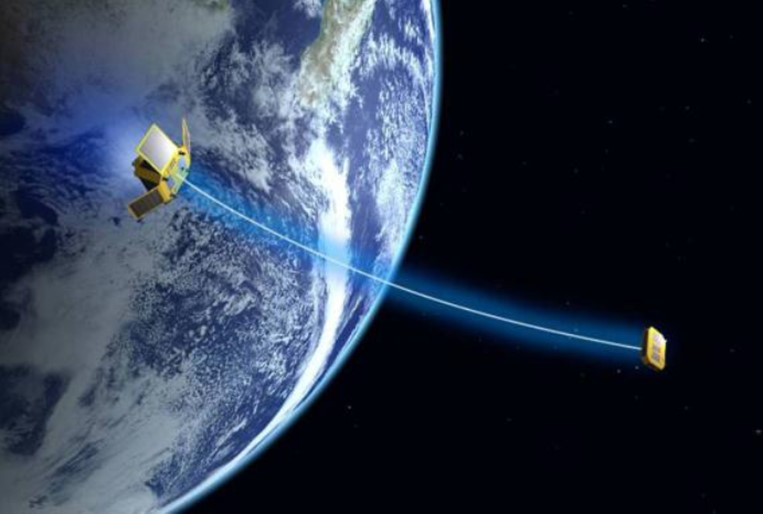
\includegraphics[width=\linewidth]{figures/EDTbasci}
				\caption{EDT系统的原理示意图}
			\end{figure}
		\end{center}
	\end{column}
\end{columns}
\end{frame}


%%%%%%%%%%%%%%%%%%%%%%%%%%%%%%%%%%%%%%%%%%%%%%%%%
\tableofcontentslide

%%%%%%%%%%%%%%%%%%%%%%%%%%%%%%%%%%%%%%%%%%%%%%%%%
\section{研究背景}
\tableofcontentslide[sectionstyle={show/shaded},subsectionstyle={show/show/hide},subsubsectionstyle={hide/hide/hide/hide}]
\subsection{空间碎片现状}
\begin{frame}{空间碎片}
\begin{columns}
	\begin{column}{.48\linewidth}
		1957 年至今, 已有20 多个国家和国际组织先后进行了4800多次航天发射与飞行, 送入空间的物体超过6000个, 其中仍有大约三分之一遗留在空间沿轨道飞行,其他的因丧失功能而变成了空间垃圾。同时,已发生过240 余次在轨航天器或火箭载体爆炸/撞击(破碎)事件,产生了数量众多的空间垃圾。
	\end{column}
	\begin{column}{.5\linewidth}
		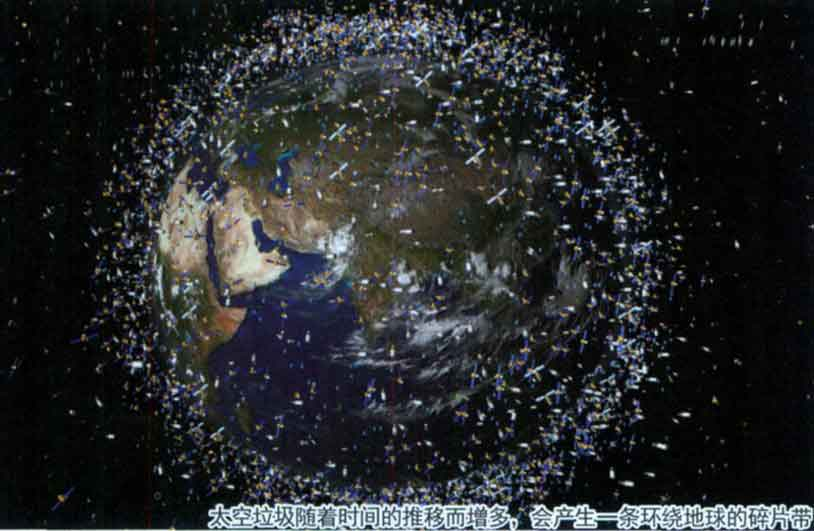
\includegraphics[width=\linewidth]{figures/debristatus}
		\begin{alertblock}{危!}
			在近地轨道,若其数量达到饱和状态,则意味着碎片与卫星相碰概率增大,甚至有可能由于碰撞而发生连锁反应,使得轨道资源成为废墟
		\end{alertblock}
	\end{column}
\end{columns}
\end{frame}
\subsection{空间碎片的危害}
\begin{frame}{空间碎片的来源}
\begin{itemize}
\item 意外解体和有意自毁产生长期存在的碎片
\item \alert{运载火箭轨道级和航天器运行过程中有意分离的碎片}
\item 碰撞和连锁碰撞产生的碎片
\end{itemize}
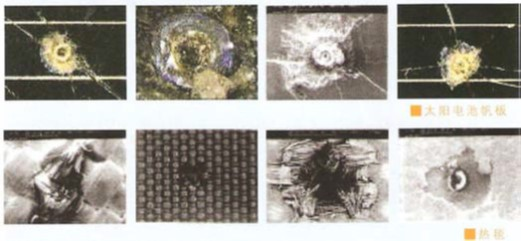
\includegraphics[width=\linewidth]{figures/debrisharm}
\end{frame}

\subsection{电动力绳系的应用前景}
\begin{frame}{EDT销毁空间碎片应用}
电动力绳系清除太空垃圾具有可行性,且重要一点成本较低,具体应用:
\begin{itemize}
\item 在未来的卫星平台或火箭第三级加装一种小型的EDT系统,在卫星寿命结束或第三级脱落后,加速报废卫星进入销毁轨道,从而控制未来在轨垃圾的数量
\item 发展电绳系推进技术与非合作目标捕获技术相结合的卫星平台,它通过捕获在轨垃圾、碎片后,通过电绳系推进变轨,将碎片“搬运”至地球销毁轨道,然后再通过电绳系推进该卫星平台又升轨回到原先轨道,再执行下一次的捕获销毁任务
\end{itemize}
\end{frame}
\section{电动力绳系推进技术}
\tableofcontentslide[sectionstyle={show/shaded},subsectionstyle={show/show/hide},subsubsectionstyle={hide/hide/hide/hide}]
\subsection{EDT系统架构}
\begin{frame}{电动力绳降轨系统组成}
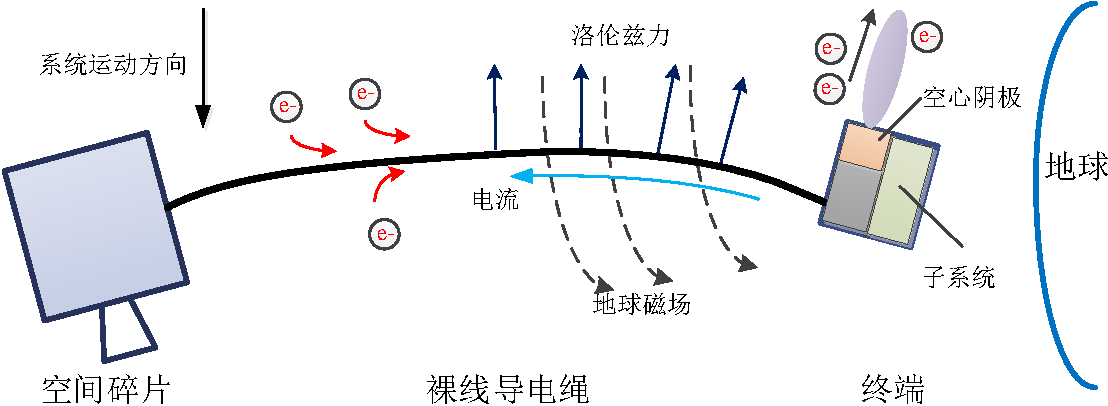
\includegraphics[width=\linewidth]{figures/deorbitdemo}
\begin{itemize}
\item 电子收集装置
\item 电子释放装置
\item 导电系绳
\end{itemize}
\end{frame}

\begin{frame}{EDT系统硬件架构}
\begin{columns}
\begin{column}{.6\linewidth}
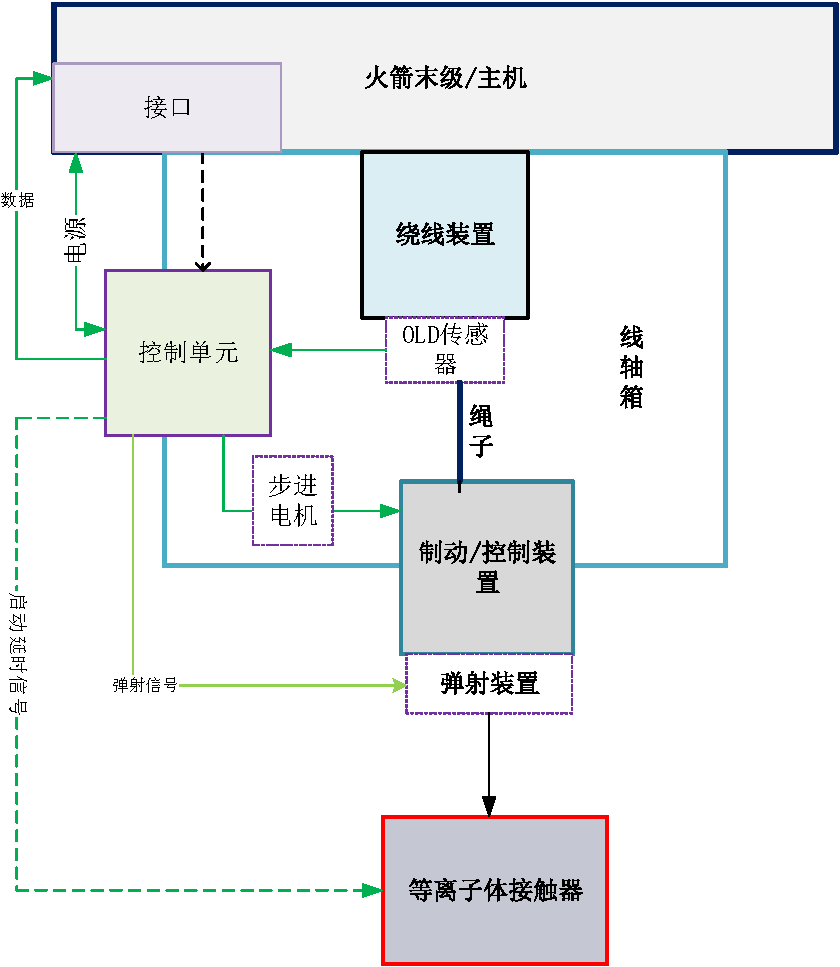
\includegraphics[width=\linewidth]{figures/hardwaredemo}
\end{column}%
\hfil
\begin{column}{.3\linewidth}
\begin{block}{主要模块}
\begin{itemize}
\item 储线模块
\item 制动控制模块
\item 接触器模块
\end{itemize}
\end{block}
\end{column}
\end{columns}
\end{frame}

\subsection{各组件简介}
\begin{frame}[c]{电子收集装置}
\begin{columns}
\begin{column}{.5\linewidth}
\begin{block}{球形结构}
\centering
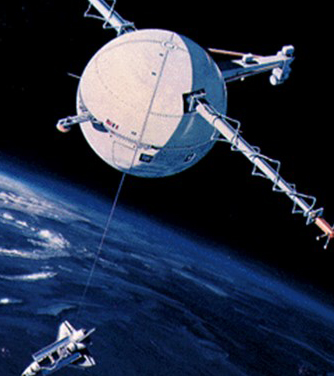
\includegraphics[width=0.7\linewidth]{figures/spherestruc}
\begin{itemize}
\item 吸收电子效率低;
\item 系统质量大
\end{itemize}
\end{block}
\end{column}%
\hfil
\begin{column}{.5\linewidth}
\begin{block}{裸线绳结构}
\centering
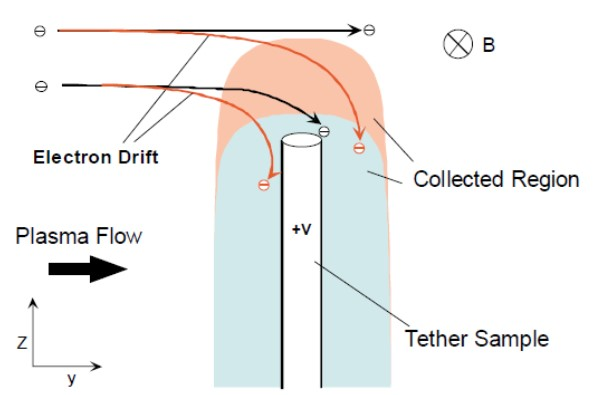
\includegraphics[width=0.8\linewidth]{figures/bareoml}
\begin{itemize}
\item 收集电子效率高;
\item  系统总质量小;
\item Sanmartin 提出把导电绳裸露部分自身作为阳极收集电子。

\end{itemize}
\end{block}
\end{column}
\end{columns}
\end{frame}


\begin{frame}[c]{电子释放装置}
\begin{columns}
\begin{column}{.5\linewidth}
\begin{block}{三大结构}
\begin{itemize}
\item 热极电子枪(TC);
\item 场发射阵列(FEAs);
\item \alert{空心阴极等离子体接触器(HCPC)}
\end{itemize}
\end{block}
\end{column}%
\hfil
\begin{column}{.5\linewidth}

\centering
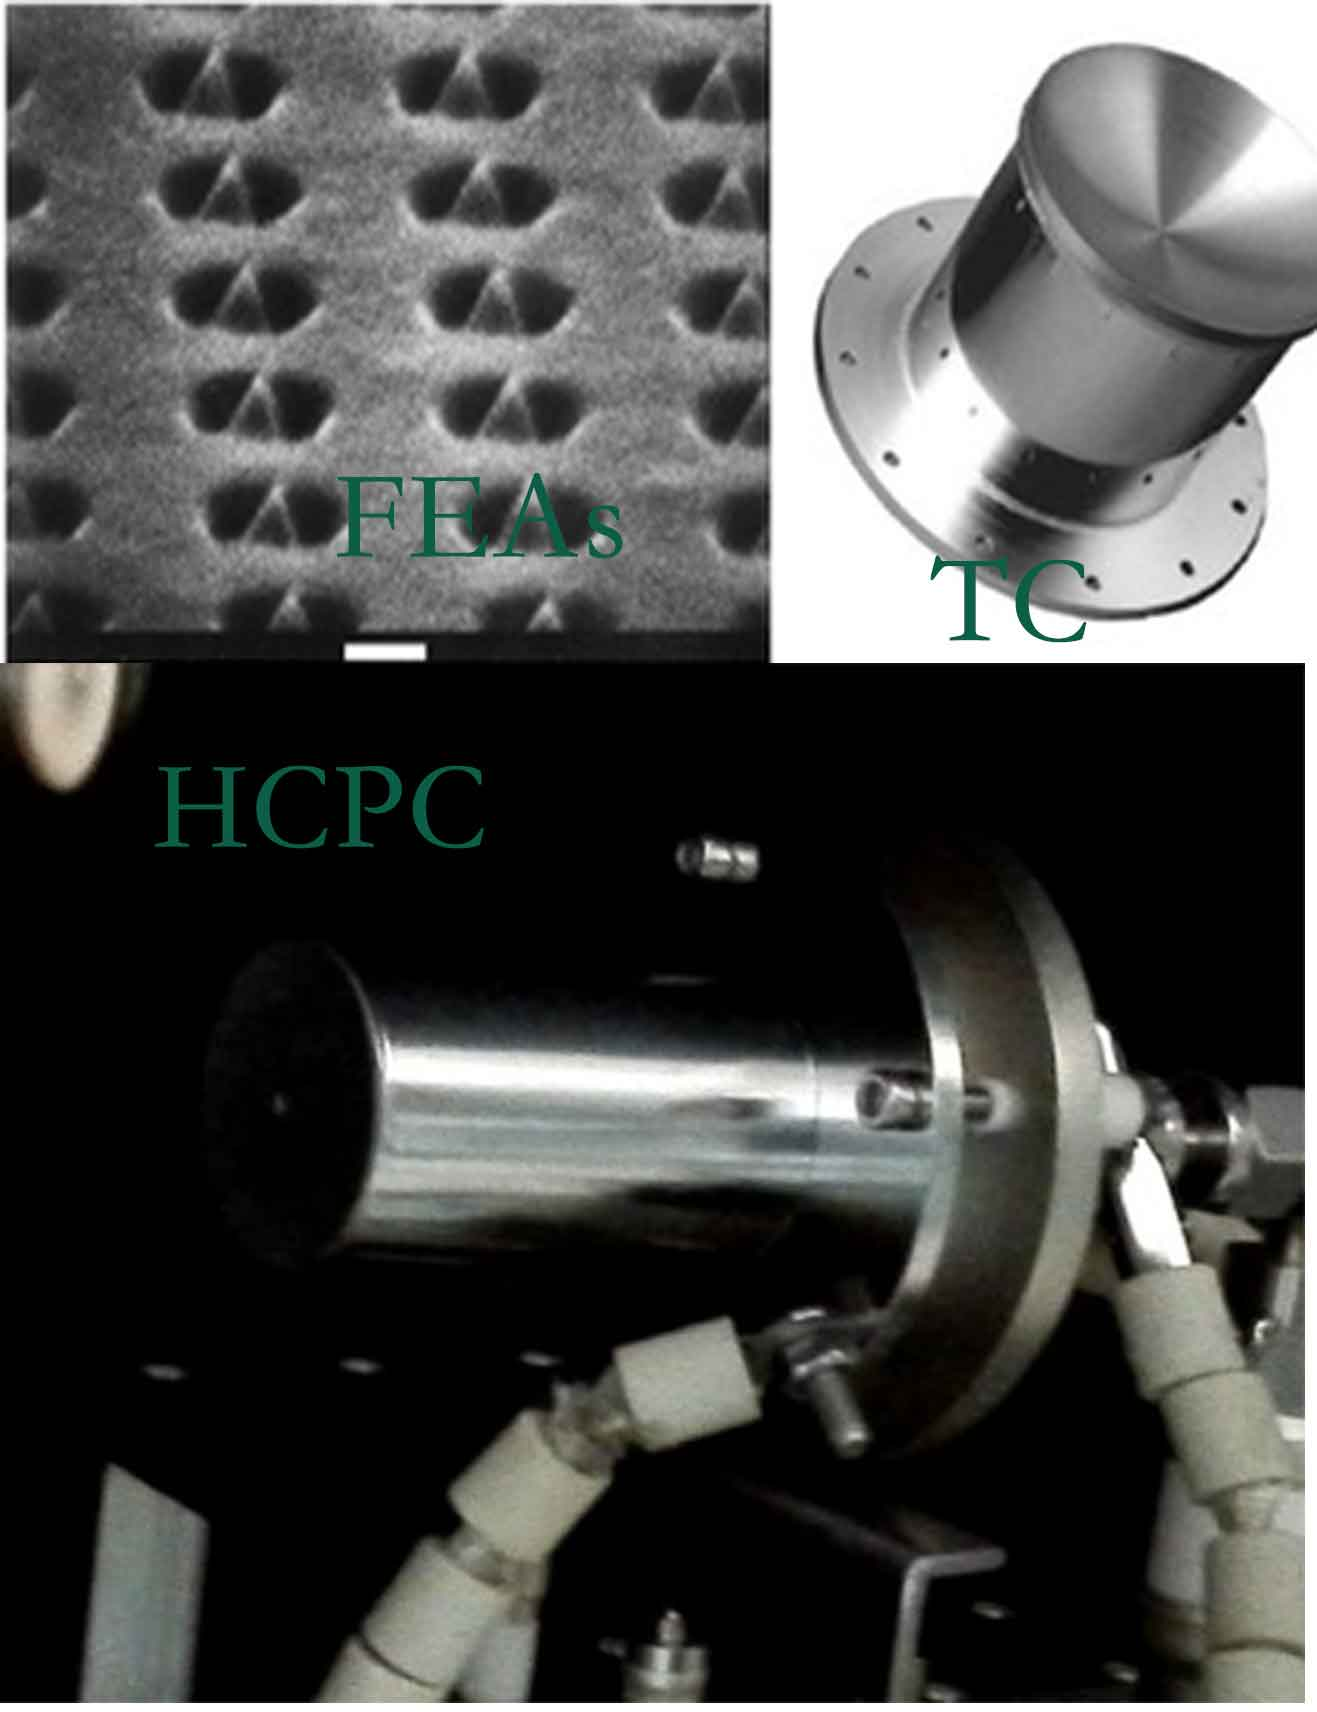
\includegraphics[width=\linewidth]{figures/emitter}
\end{column}
\end{columns}
\end{frame}


\begin{frame}[c]{导电系绳}
导电绳子电动力绳系的核心部件,空间电动力绳系因生存环境复杂需要对绳系的强度、抗干扰能力等有较高的要求,因此学者们提出了多种系绳的结构。
\centering
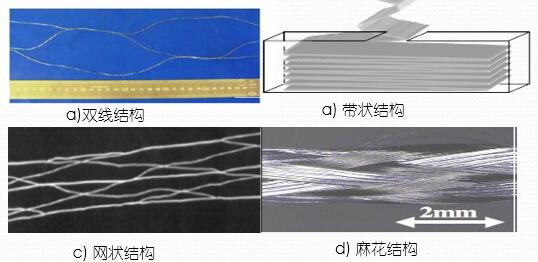
\includegraphics[width=0.9\linewidth]{figures/baretether}
\end{frame}
%-=-=-=-=-=-=-=-=-=-=-=-=-=-=-=-=-=-=-=-=-=-=-=-=
%
%	可行性分析
%
%-=-=-=-=-=-=-=-=-=-=-=-=-=-=-=-=-=-=-=-=-=-=-=-=
\section{EDT技术可行性分析}
\tableofcontentslide[sectionstyle={show/shaded},subsectionstyle={show/show/hide},subsubsectionstyle={hide/hide/hide/hide}]
\subsection{EDT在轨实验验证}
\begin{frame}[label=online]{国外在轨实验}
% Table generated by Excel2LaTeX from sheet 'Sheet1'
\footnotesize \setlength{\tabcolsep}{0.1pt}
\centering
\resizebox{\textwidth}{!}{
\begin{tabular}{ccccccr}
\toprule
\rowcolor[rgb]{ 1,  .949,  .8} \multicolumn{1}{c}{\textcolor[rgb]{ .612,  .341,  0}{研究机构}} & \textcolor[rgb]{ .612,  .341,  0}{发射日期} & \textcolor[rgb]{ .612,  .341,  0}{项目名称} & \multicolumn{1}{c}{\textcolor[rgb]{ .612,  .341,  0}{绳子长度}} & \textcolor[rgb]{ .612,  .341,  0}{主要研究} & \textcolor[rgb]{ .612,  .341,  0}{成功与否} & \multicolumn{1}{c}{\textcolor[rgb]{ .612,  .341,  0}{备注}} \\
\midrule
NASA  & 1966  & Gemini 11 & 0.036 & 人造重力  & 是     & \multicolumn{1}{c}{旋转保持0.15rpm} \\
NASA  & 1966  & Gemini 12 & 0.44  & 重力梯度稳定 & 是     & \multicolumn{1}{c}{人工手动控制} \\
NASA/ISAS & 1985  & Charge‐2 & 0.426 & 电子的收集与发射 & 是     &  \\
NASA/ISAS & 1992  & CHARGE - 2B & 0.4   & 电子的收集与发射 & 是     &  \\
CSA   & 1989  & Oedipus‐A & 0.959 & 等离子体研究 & 是     &  \\
CSA   & 1995  & Oedipus‐C & 1.174 & 等离子体研究 & ——    &  \\
\rowcolor[rgb]{ .867,  .922,  .969} \textcolor[rgb]{ .753,  0,  0}{NASA/ISAS} & \textcolor[rgb]{ .753,  0,  0}{1992} & \textcolor[rgb]{ .753,  0,  0}{TSS‐1} & \textcolor[rgb]{ .753,  0,  0}{0.26} & \textcolor[rgb]{ .753,  0,  0}{电动力及电流产生} & \textcolor[rgb]{ .753,  0,  0}{否} & \multicolumn{1}{c}{\textcolor[rgb]{ .753,  0,  0}{绳子被卡住}} \\
\rowcolor[rgb]{ .867,  .922,  .969} \textcolor[rgb]{ .753,  0,  0}{NASA/ISAS} & \textcolor[rgb]{ .753,  0,  0}{1996} & \textcolor[rgb]{ .753,  0,  0}{TSS‐1R} & \textcolor[rgb]{ .753,  0,  0}{19.6} & \textcolor[rgb]{ .753,  0,  0}{力及电流产生} & \textcolor[rgb]{ .753,  0,  0}{大部分是} & \multicolumn{1}{c}{\textcolor[rgb]{ .753,  0,  0}{绳子后来被碎片隔断}} \\
\rowcolor[rgb]{ .867,  .922,  .969} \textcolor[rgb]{ .753,  0,  0}{NASA} & \textcolor[rgb]{ .753,  0,  0}{1993} & \textcolor[rgb]{ .753,  0,  0}{PMG} & \textcolor[rgb]{ .753,  0,  0}{0.5} & \textcolor[rgb]{ .753,  0,  0}{电流和推力特性} & \textcolor[rgb]{ .753,  0,  0}{是} & \multicolumn{1}{c}{\textcolor[rgb]{ .753,  0,  0}{7个小时的飞行}} \\
NASA  & 1993  & SEDS‐1 & 20    & 绳系选择,切断控制 & 是     & \multicolumn{1}{c}{绳子后被切断} \\
NASA  & 1994  & SEDS‐2 & 19.7  & 绳系的控制、伸展 & 是     &  \\
NRL   & 1996  & TiPS  & 4     & 绳系的生存能力及稳定性 & 是     &  \\
\rowcolor[rgb]{ .867,  .922,  .969} \textcolor[rgb]{ .753,  0,  0}{NASA} & \textcolor[rgb]{ .753,  0,  0}{2005} & \textcolor[rgb]{ .753,  0,  0}{ProSEDS} & \textcolor[rgb]{ .753,  0,  0}{19} & \textcolor[rgb]{ .753,  0,  0}{电动力对废弃卫星降轨} & \textcolor[rgb]{ .753,  0,  0}{任务取消} & \multicolumn{1}{c}{\textcolor[rgb]{ .753,  0,  0}{空间站安全取消}} \\
ESA   & 1997  & YES   & 35    & 旋转、再轨 & 否     & \multicolumn{1}{c}{轨道选择不当} \\
ESA   & 2007  & YES2  & 31.7  & 航天器的精确再轨 & 大部分是  & \multicolumn{1}{c}{过度绳系展开} \\
NRO   & 1998  & ATeX  & 0.02 of 6.2 & 稳定性和存活率 & 否     & \multicolumn{1}{c}{S/W阻止展开} \\
\rowcolor[rgb]{ .867,  .922,  .969} \textcolor[rgb]{ .753,  0,  0}{TUI/IDC} & \textcolor[rgb]{ .753,  0,  0}{2007} & \textcolor[rgb]{ .753,  0,  0}{MAST} & \textcolor[rgb]{ .753,  0,  0}{1} & \textcolor[rgb]{ .753,  0,  0}{动力学数据采集} & \textcolor[rgb]{ .753,  0,  0}{否} & \multicolumn{1}{c}{\textcolor[rgb]{ .753,  0,  0}{没有展开}} \\
\rowcolor[rgb]{ .867,  .922,  .969} \textcolor[rgb]{ .753,  0,  0}{JAXA} & \textcolor[rgb]{ .753,  0,  0}{2010} & \textcolor[rgb]{ .753,  0,  0}{T‐REX} & \textcolor[rgb]{ .753,  0,  0}{0.3} & \textcolor[rgb]{ .753,  0,  0}{带绳展开、HCPC及OML验证} & \textcolor[rgb]{ .753,  0,  0}{大部分是} & \multicolumn{1}{c}{\textcolor[rgb]{ .753,  0,  0}{亚轨道运行成功}} \\
\rowcolor[rgb]{ .867,  .922,  .969} \textcolor[rgb]{ .753,  0,  0}{JAXA} & \textcolor[rgb]{ .753,  0,  0}{2017} & \textcolor[rgb]{ .753,  0,  0}{HTV6} & \textcolor[rgb]{ .753,  0,  0}{0.7} & \textcolor[rgb]{ .753,  0,  0}{空间碎片离轨} & \textcolor[rgb]{ .753,  0,  0}{失败} & \textcolor[rgb]{ .753,  0,  0}{释放机构出错} \\
\bottomrule
\end{tabular}}
\end{frame}

\subsection{国外EDT项目}
\begin{frame}[c]{国外重点实验介绍}
\vspace{-10pt}
\centering
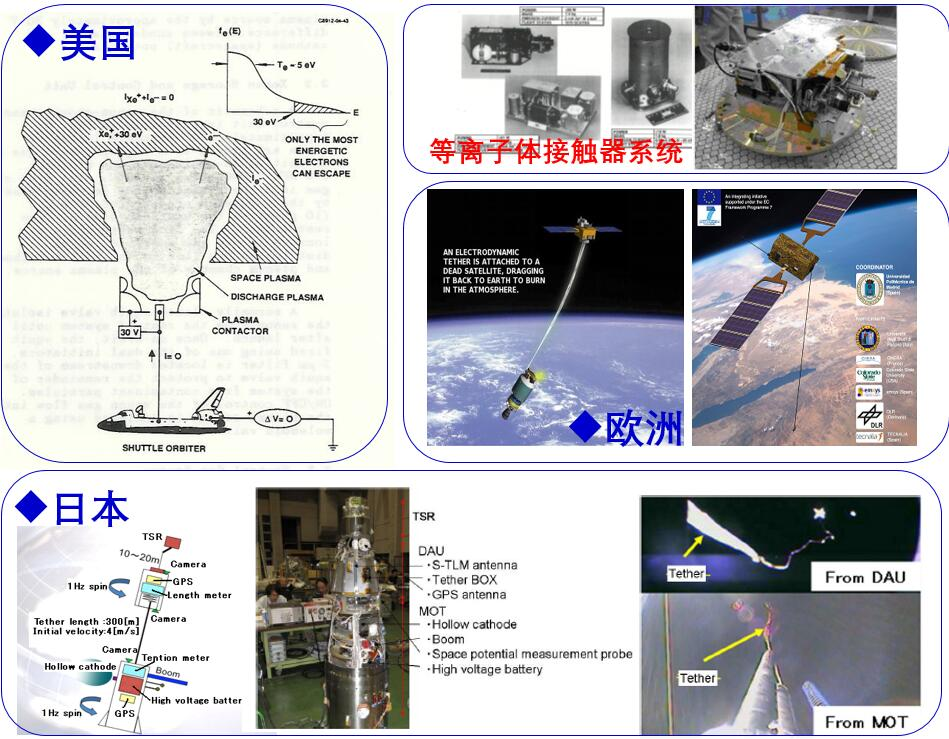
\includegraphics[width=0.9\linewidth]{figures/onlinelab}
\end{frame}
\begin{frame}{国内研究状况}
国内目前并没有开展关于空间电动力绳系的在轨实验。

	\begin{itemize}
		\item 主要集中在动力学和模拟仿真阶段;
		\item 南京航空航天大学利用气浮平台实验;
		
		\item 北京理工大学进行核心部件空心阴极等离子体接触器的地面试验,研究实际空心阴极的实际放电特性,研制模型样机,搭建总体释放实验平台。
		
		\begin{center}
			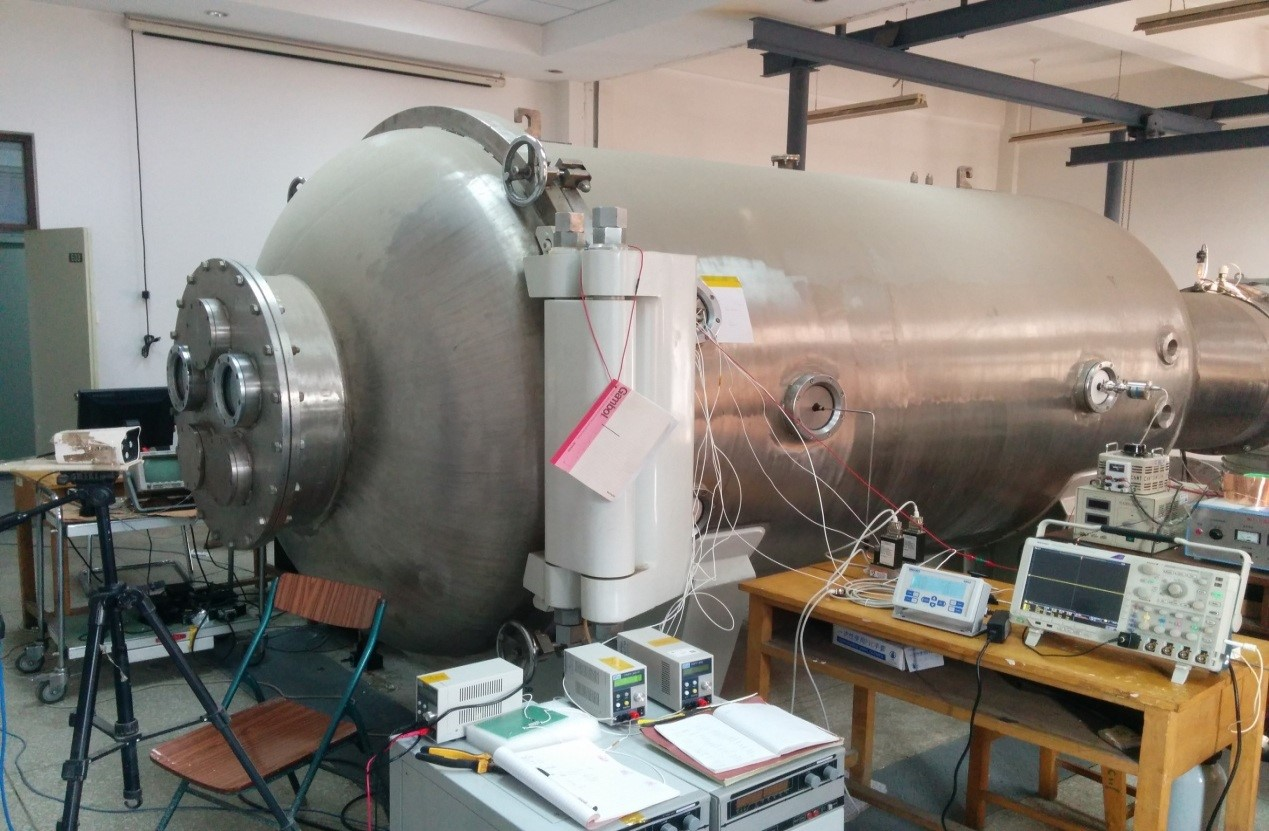
\includegraphics[width=0.5\linewidth]{figures/dimianshiyan}
		\end{center}  
	\end{itemize}
\end{frame}

\begin{frame}{可行性分析总结}
\begin{itemize}
\item 在轨道实验验证了绳系中电流、洛伦兹力的产生的可行性;
\item 应用具有可靠性(Tips实验,在轨服役10年),基本原理和实验上的可行性;
\item 几次重大的失败的在轨试验是由于机械结构设计上存在缺陷,而不是基本理论的错误;
\item 目前尚未有降轨销毁碎片的成功案例,日本的HIV6实验由于释放机构设计缺陷而失败。
\end{itemize}
\textgoto{online}{在轨实验统计表}
\end{frame}

\section{电动力绳降轨模型}
\tableofcontentslide[sectionstyle={show/shaded},subsectionstyle={show/show/hide},subsubsectionstyle={hide/hide/hide/hide}]
\begin{frame}{电动力绳系动力学模型}
在仿真中,EDT系统假设为二力杆刚体绕地球运动,计算变轨过程使用了相对二体运动轨道计算原理:
\[\bm{\ddot r}=  - \frac{\mu }{r^3} \bm{ r} + \frac{\textbf F}{m_2}\]
式中,$\ddot{r}$  为系统在地心惯性坐标系中的加速度矢量, $r$为卫星到地心的距离, $\mu$ 为地球引力常数,$F$表示作用在系统上的摄动力,这里仅考虑洛伦兹力和大气阻力。%式是一个六阶的的非线性微分方程,在某个时刻$t$下给定初始位置和速度,通过龙格-库塔(Runge-Kutta)数值求解方法,计算下一个时刻系统的参数。
\end{frame}

\begin{frame}{电子收集模型}
裸线绳系收集的理论很多,其中目前公认较好的描述该现象的理论是轨道限制理论(简称OML理论)。可由OML理论推导出电动力绳系上绳长为$l$ 的电流变化率:
\[
\dfrac{dI}{dl}=\begin{cases}
\dfrac{e N_e p}{\pi}\sqrt{\smash[bt]{\dfrac{2e\Delta V}{m_e}}}  &\text{$ V_t-V_p>0$}\\[15pt]
-\dfrac{e N_i p}{\pi}\sqrt{\dfrac{-2e\Delta V}{m_i}}  &\text{$ V_t-V_p<0$}\\
0 &\text{其他}
\end{cases}\]
式中, $ e $为电子电荷, $ N_e $为电子密度,$ l $ 为系绳的周长, $V_t$为系绳上的电势, $V_p$为空间等离子体电势, $m_e$为电子的质量。
\end{frame}

\begin{frame}{电子收集模型}
\begin{columns}
\begin{column}{.4\linewidth}
系绳上的电势沿一段长度 的绳子变化可由式给出:
\begin{gather}
\frac{\mathrm{d} V_t } {dy} =\frac{I} {\sigma S }\notag\\
\frac{\mathrm{d}V_p }  {dy}+E_m =0\notag\\
\frac{\mathrm{d} \Delta V } {\mathrm{d} y }  =\frac{\mathrm{d} V_t} {\mathrm {d} y}-\frac{\mathrm{d} V_p} {\mathrm{d}y }\notag
\end{gather}\label{eq:voltage and current}
$\sigma$绳子材料的导电率,$S$为绳子的截面面积。$E_m$ 为绳子的感应电场强度。%为了求解式中方程组,可由边界条件:
\end{column}
\begin{column}{.7\linewidth}
\centering
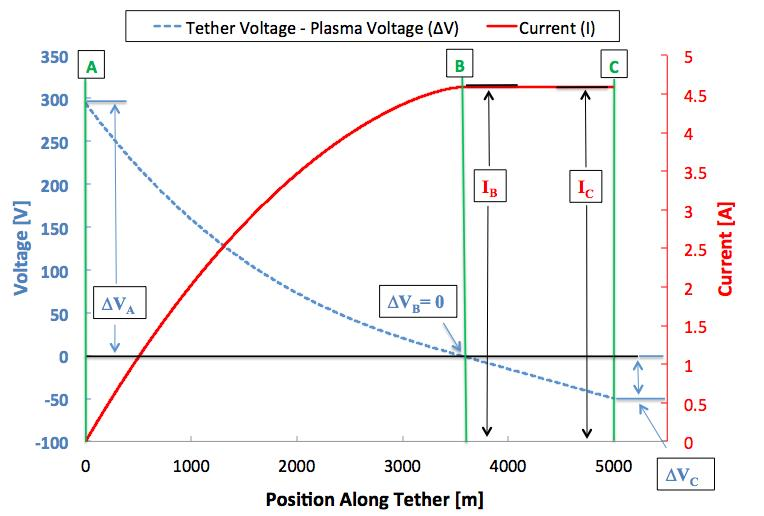
\includegraphics[width=\linewidth]{figures/IVdemo}
\end{column}
\end{columns}
\end{frame}

\begin{frame}{电子收集模型}
为了求解式中方程组,可由边界条件:
\[
\begin{cases}
V_t  \, \vert_ {y=0} =V_A \\
I \, \vert_ {y=0 } =0 \\
V_p \,  \vert_ {y=0} =0
\end{cases}
\]

\[
\begin{cases}
V_t  \, \vert_ {l=l} =V_p  \, \vert_ {l=l} -V_c \\
V_p \,  \vert_ {l=l} =E_m l \\
I \, \vert_ {l=l } =I_c
\end{cases}
\]
式中,$V_A$为绳子$AC$的A端电势,$V_C$ 为绳子$AC$的C端电势,即等效于电离子接触器发射端的电势$I_C$为发射电流。
\end{frame}

\begin{frame}{HCPC阴极电流-电压曲线}
$V_C$ 为绳子$AC$的C端电势,该边界条件可由实际的HCPC实验测得I-V曲线:
\centering
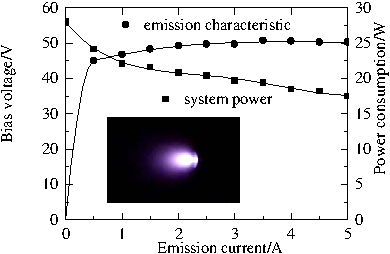
\includegraphics[width=0.9\linewidth]{figures/emissioncurrent}
\end{frame}

\begin{frame}{洛伦兹力计算模型}
\begin{itemize}
\item 电动力绳系在地磁场中运动时,产生感应出电动势
\[\bm{E}_m=\bm{V}_r \times\bm{B}\]
\item 绳索与周围电离层相互耦合产生电流:
\[I=\frac{E}{R}\]
\item 导电绳在电磁场中运动,产生洛仑兹力:
\[\bm{F}=\int_0^l  \bm{I}dl \times \bm{B}\]
\end{itemize}
估算:同步轨道上,$v=7.5\si{km/s}$,$B=20\si{\mu T}$,产生$E=15\si{V/m}$,电流$I=10-20\si{A}$,洛伦兹力$F=0.5-1N$
\end{frame}

\section{化学火箭发动机推进系统的降轨计算}
\tableofcontentslide[sectionstyle={show/shaded},subsectionstyle={show/show/hide},subsubsectionstyle={hide/hide/hide/hide}]
\begin{frame}{化学火箭发动机推进系统降轨模型}
采用传统的固体火箭发动机推进计算方法,参照轨道动力学二体运动模型,采用理想霍曼转移轨道降轨

\centering
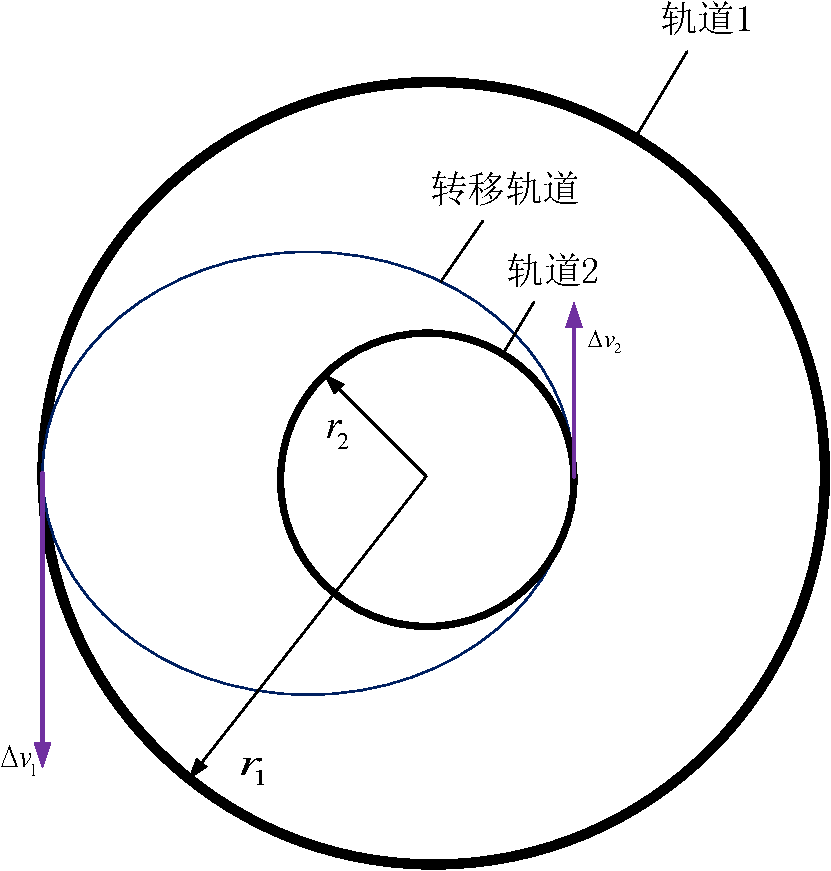
\includegraphics[width=0.5\linewidth]{figures/Hoffmantansfer}
\end{frame}

\begin{frame}{计算方法}
\begin{itemize}
\item 两次变轨速度增量:
\begin{gather}
\Delta {v_1} = \sqrt {\frac{\mu }{{{r_2}}}} (\sqrt {\frac{{2{r_1}}}{{{r_1} + {r_2}}}}  - 1) \notag\\
\Delta {v_2} = \sqrt {\frac{\mu }{{{r_1}}}} (1{\rm{ - }}\sqrt {\frac{{2{r_1}}}{{{r_1} + {r_2}}}} )\notag
\end{gather}
\item 由开普勒第三定律可得变轨时间:
\begin{equation}
\Delta t = \frac{1}{2}\sqrt {\frac{{4{\pi ^2}a_H^3}}{\mu }}  = \pi \sqrt {\frac{{{{({r_1} + {r_2})}^3}}}{{g\mu }}}\notag
\end{equation}\label{eq:time}
\item 化学推进系统的推进剂的质量:
\begin{equation}
{M_p} = \frac{(\Delta {v_1} + \Delta {v_2})m}{{{I_{sp}}}}\notag
\end{equation}\label{eq:M_p}
\end{itemize}
\end{frame}

\section{电动力绳系降轨性能分析}
\tableofcontentslide[sectionstyle={show/shaded},subsectionstyle={show/show/hide},subsubsectionstyle={hide/hide/hide/hide}]
\subsection{仿真条件设定}
\subsection{降轨空间碎片参数设定}
\begin{frame}{降轨碎片模型参数设定}
\begin{columns}
\begin{column}{.5\linewidth}
\begin{block}{参数设定}
\begin{itemize}
\item 轨道参数:$0^\circ$倾角,高度$850\si{km}-150\si{km}$;
\item 导电绳参数:铝质绳长度$5\si{km}$,直径$1\si{mm}$;
\item 地球环境模型:IRI(2007)模型、IGRI2012,低于300km的大气阻力模型
\item 系统质量:碎片质量$1000\si{kg}$,EDT系统质量约$114\si{kg}$
\end{itemize}
\end{block}
\end{column}%
\hfil
\begin{column}{.5\linewidth}

\centering
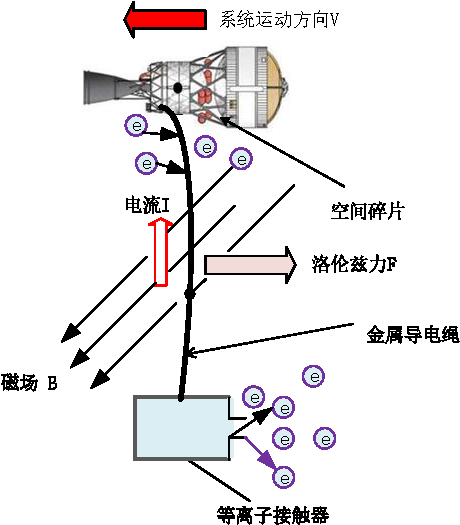
\includegraphics[width=\linewidth]{figures/EDTsystem}
\end{column}
\end{columns}
\end{frame}
\subsection{性能分析}
\begin{frame}{EDT高度与时间的变化}
\begin{minipage}{0.6\textwidth}
\begin{center}
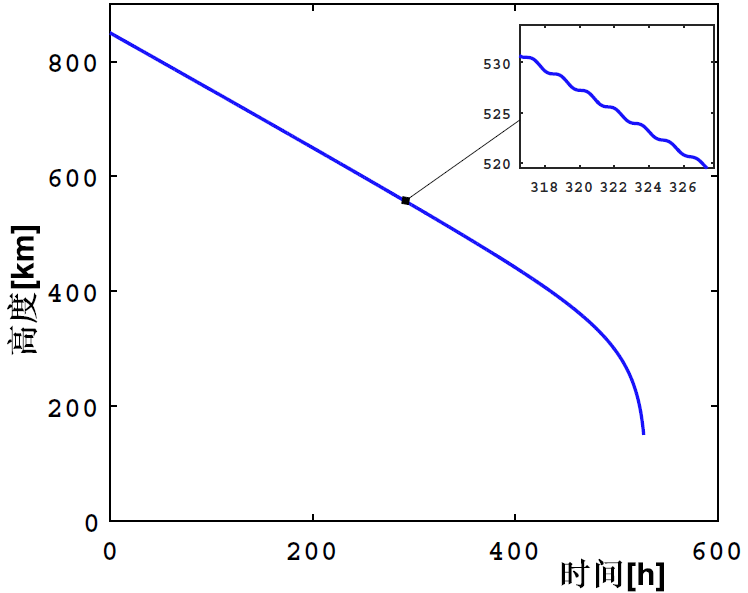
\includegraphics[width=1\linewidth]{figures/tHg}
\end{center}
\end{minipage}%
\begin{minipage}{0.4\textwidth}
\begin{itemize}
\item 降轨消耗527小时,且在高度低于300公里处的降轨速度明显加快
\item 在系统降轨过程中,系统出现振动,这和系统所受到的阻力是变化的有关。
\end{itemize}
\end{minipage}
\end{frame}


\begin{frame}{磁场与等离子体密度的变化}
\begin{minipage}{0.55\textwidth}
\begin{center}
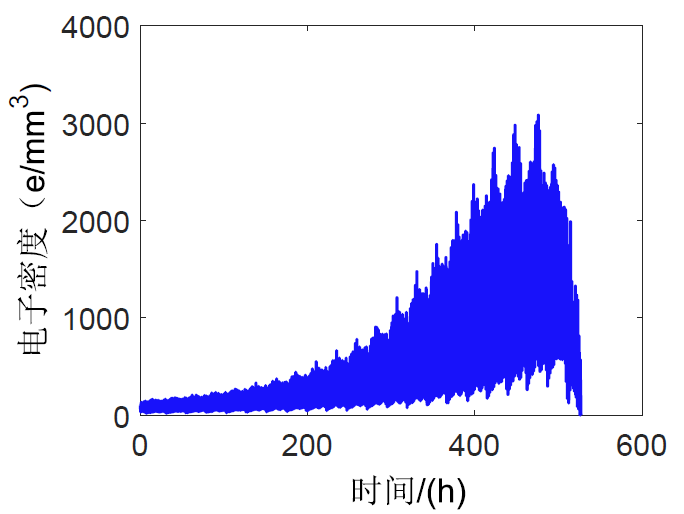
\includegraphics[width=\linewidth]{figures/tng}
\end{center}
\end{minipage}%
\begin{minipage}{0.55\textwidth}
\centering
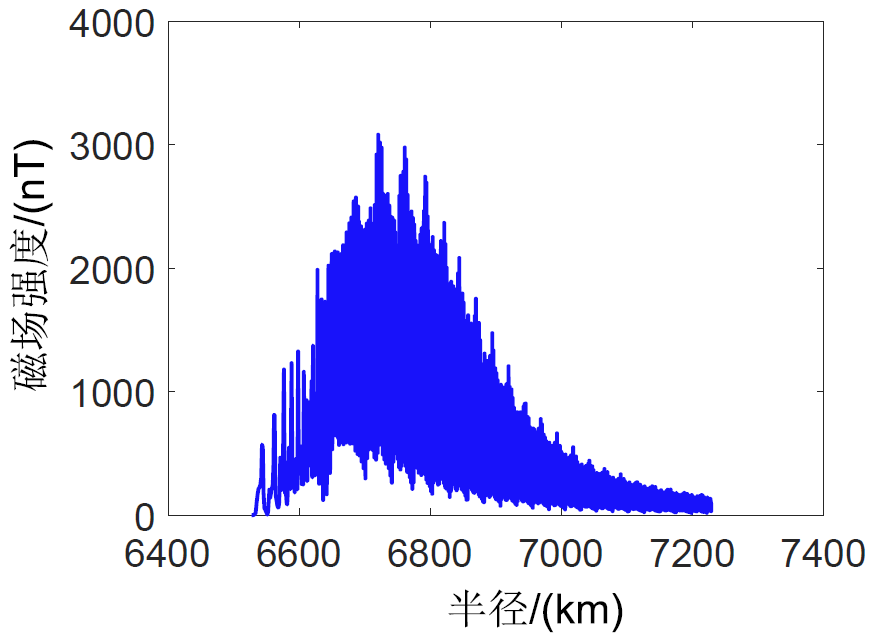
\includegraphics[width=\linewidth]{figures/tb}
\end{minipage}
推力的变化主要和地球磁场环境变化和等离子体密度相关。在磁场强度高和电子密度密集区,相应的推力越大。
\end{frame}

\begin{frame}{洛伦兹力与轨道半径的变化关系}
\begin{minipage}{0.6\textwidth}
\begin{center}
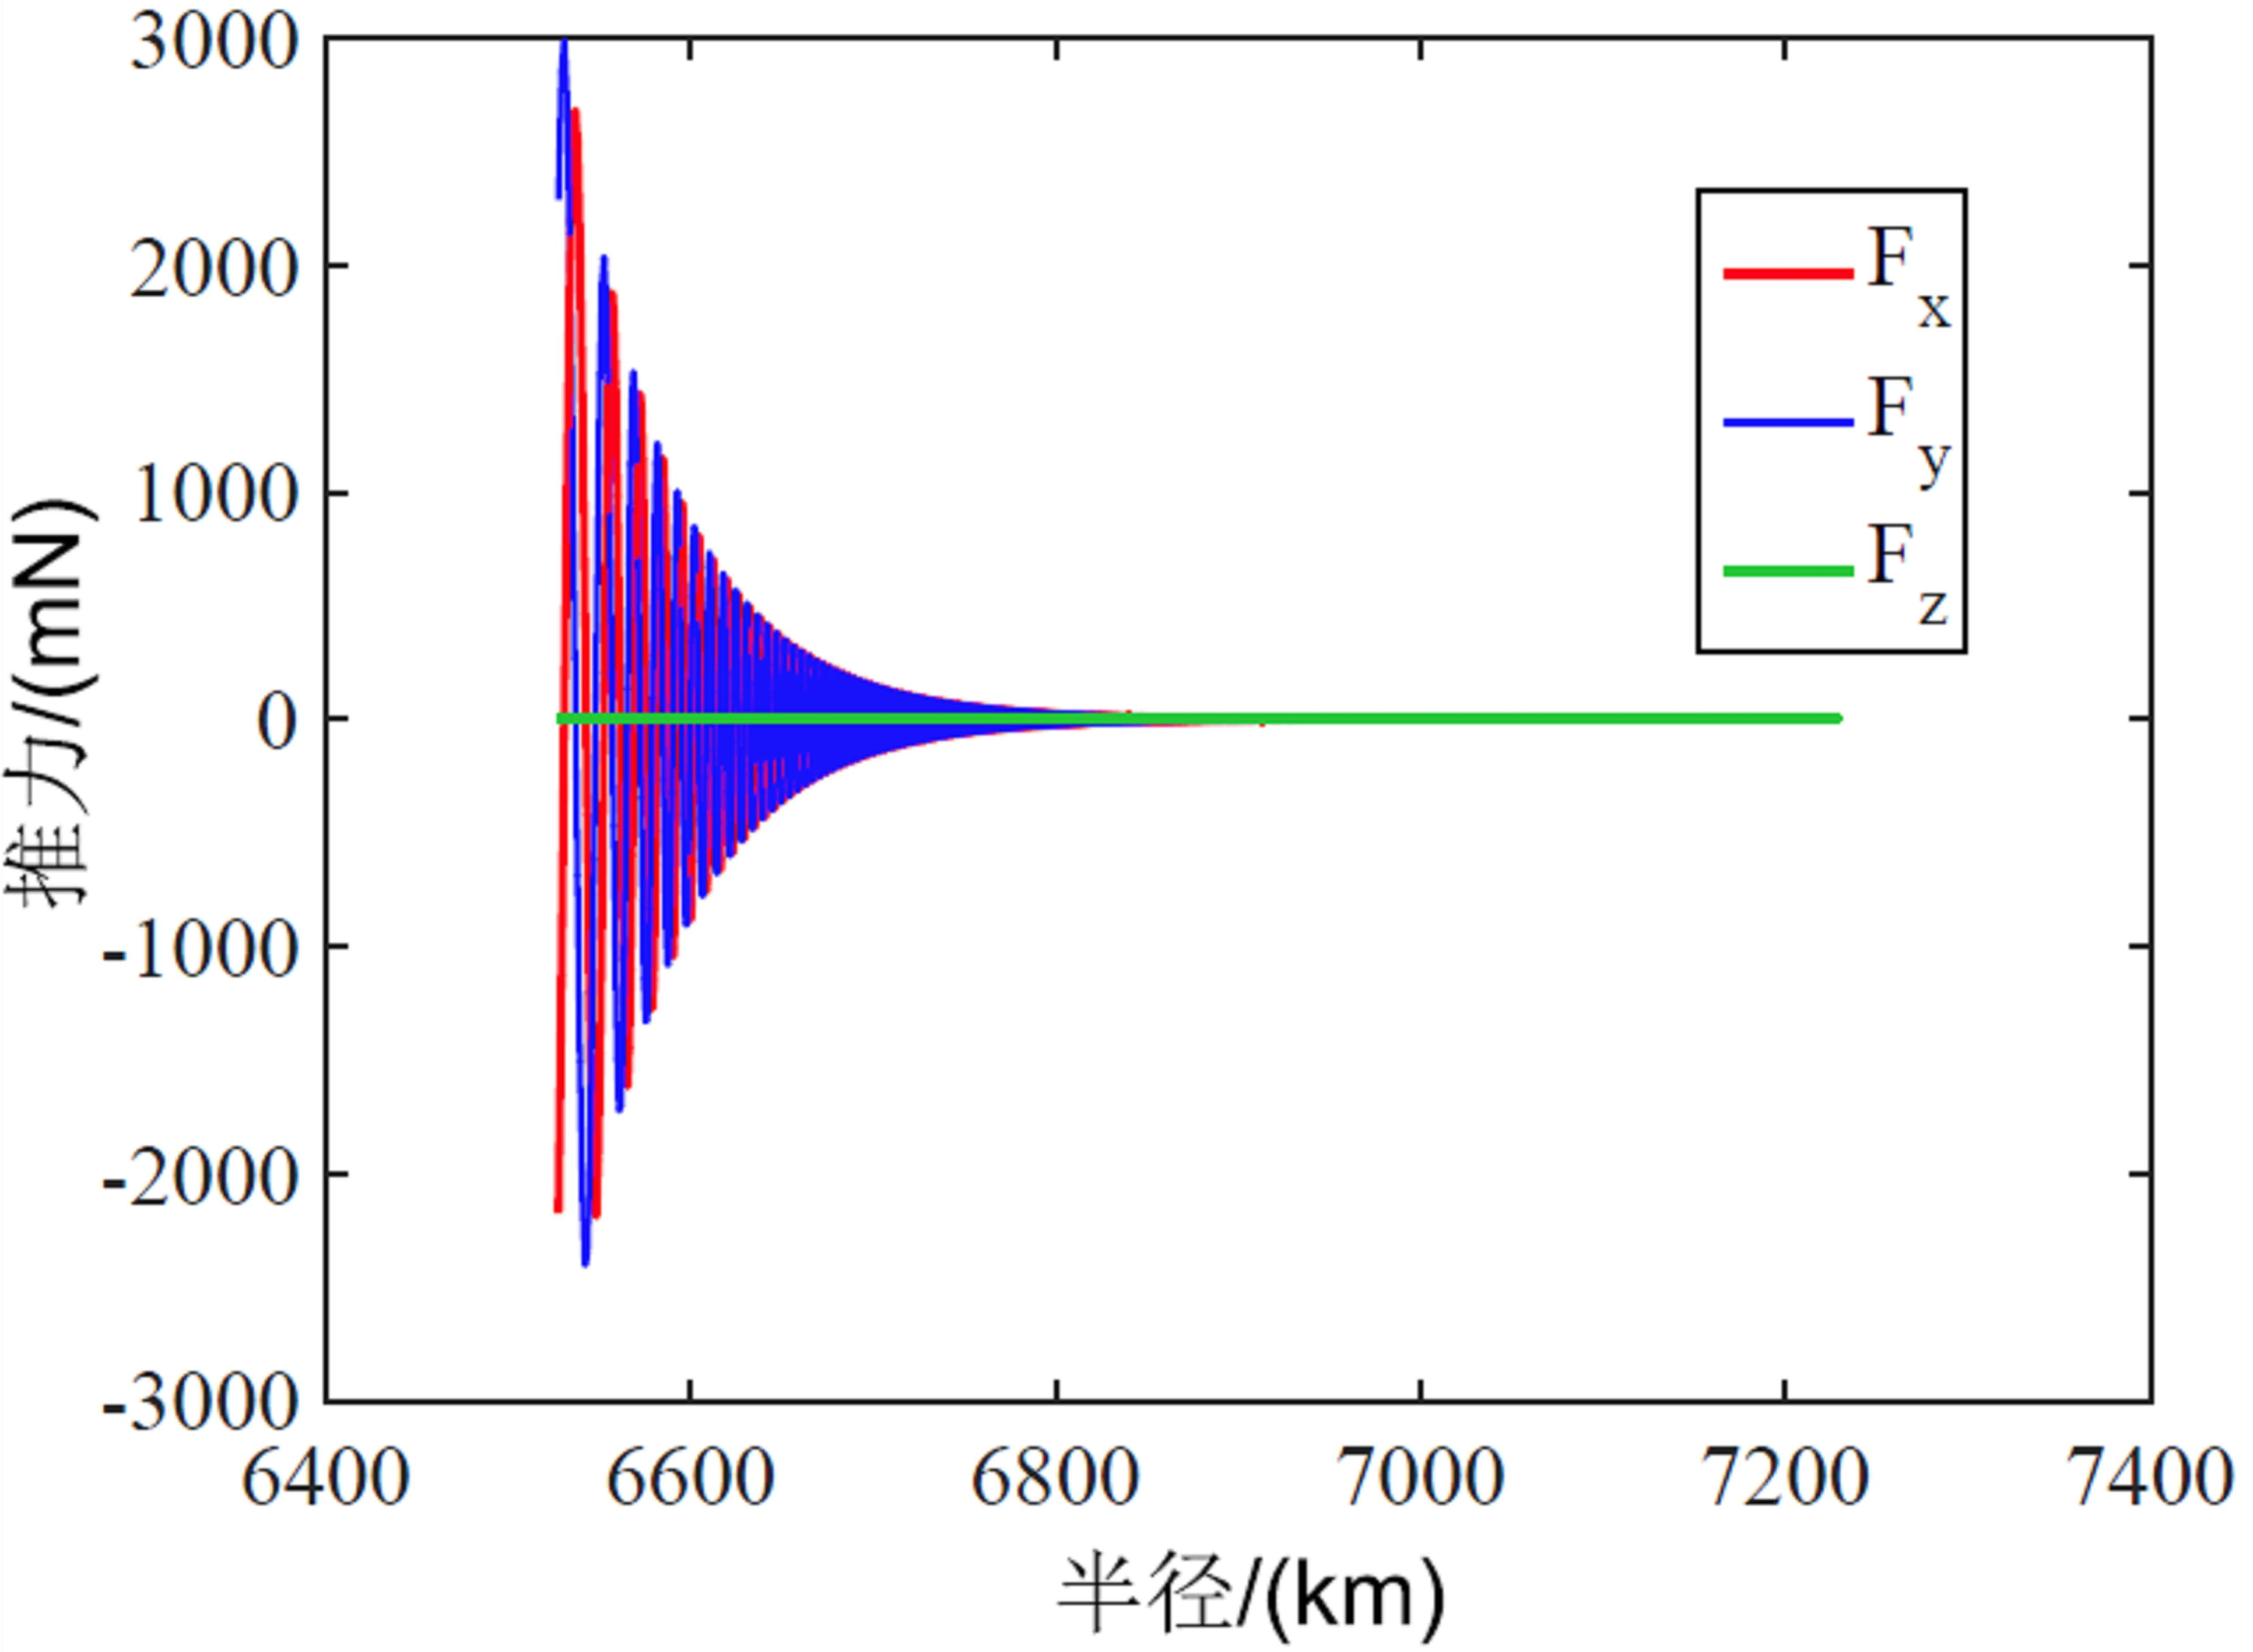
\includegraphics[width=\linewidth]{figures/tf}
\end{center}
\end{minipage}%
\begin{minipage}{0.4\textwidth}
将其沿着惯性坐标系分解,容易知道$F_y$方向上的分解为0,从图示可以看出,在$F_x$,$F_y$方向上力对称振荡,随着轨道高度的减小,效应更明显。
\end{minipage}%
\end{frame}

\begin{frame}{不同轨道倾角条件下的轨道高度的变化}
\begin{minipage}{0.6\textwidth}

\begin{center}
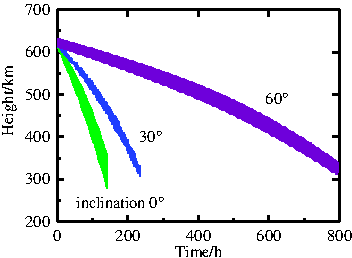
\includegraphics[width=\linewidth]{figures/th}
\end{center}
\end{minipage}%
\begin{minipage}{0.4\textwidth}
案例计算轨道倾角分别为$0^\circ$,$30^\circ$,$60^\circ$的降轨,为了节省计算机运行时间,变轨高度600-200km的变化,从图中可以看出低倾角的电动力绳降轨效果明显的多。
\end{minipage}
\end{frame}

\begin{frame}{不同轨道倾角条件下的系统洛伦兹力}
\begin{minipage}{0.6\textwidth}
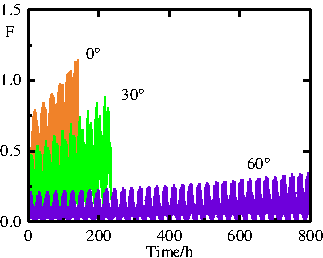
\includegraphics[width=\linewidth]{figures/f}

\end{minipage}%
\begin{minipage}{0.4\textwidth}
可以产生N级别的洛伦兹力,且随着轨道倾角的降低而增大。
同时与地球磁场和等离子成密度的变化有些正相关。
\end{minipage}%
\end{frame}

\subsection{与化学推进剂降轨的比较}
\begin{frame}{与化学火箭推进降轨的比较}
在计算化学火箭发动机性能参数时,对于化学火箭发动机,推进剂质量与发动机质量比一般限制在0.5与0.7之间,同时一般姿轨控火箭发动机的比冲范围为$250s-300s$。选取比冲为270s,并进行三组算例进行计算。
\begin{itemize}
\item 第一组算例轨道及系统参数:轨道高度850km-150km;
\item 第二组算例轨道及系统参数: 轨道高度700km-200km;
\item 第三组算例轨道及系统参数:轨道高度700km-400km;
\end{itemize}
\end{frame}

\begin{frame}[label=progressbartypes,t]{表格对比}
	\centering 第一组算例 
\resizebox{\textwidth}{!}{

\begin{tabular}{ccccc}
\toprule
比较项目       &  变轨时间($h$)   &  推进剂质量($kg$)  &  系统质量($kg$)   &  有效比冲($s$)\\
\midrule
电动力绳系统    &  527  	         &  0.013	             &  113.8	      & 27047\\
化学推进系统    & 0.79             &  159.8                &	267	          &  270 \\
\bottomrule
\end{tabular}}%
	
\centering 第二组算例 
\resizebox{\textwidth}{!}{
	 
\begin{tabular}{ccccc}
\toprule
比较项目       &  变轨时间($h$)   &  推进剂质量($kg$)  &  系统质量($kg$)   &  有效比冲($s$)\\
\midrule
电动力绳系统    &  375  	         &  0.013	             &  113.8	      & 29057\\
化学推进系统    & 0.78            &  104.5               &	174	          &  270 \\
\bottomrule
\end{tabular}}
\centering 第三组算例 
\resizebox{\textwidth}{!}{
\begin{tabular}{ccccc}
\toprule
比较项目       &  变轨时间($h$)   &  推进剂质量($kg$)  &  系统质量($kg$)   &  有效比冲($s$)\\
\midrule
电动力绳系统    &  276  	         &  0.013	             &  113.8	      & 30067\\
化学推进系统    & 0.80            &  91.6              &	151	          &  270 \\
\bottomrule
\end{tabular}}
\end{frame}

\begin{frame}{分析总结}
\begin{itemize}
\item 化学推进降轨最显著特点所需时间少,电动力绳系降轨时间相对较长,对比于自然销毁,时间短;
\item 电动力绳系的最大优点是所需推进剂量少,同样的任务,化学推进系统推进剂的质量是电动力绳系的1000多倍。随着降轨范围的增大,化学火箭发动机所需要的推进剂质量成倍增加,而电动绳系的所需要的推进剂(推进剂为氙气)几乎不变,推进系统的总质量随着轨道高度差的增大,系统的总质量显著增加,而电动力绳系的质量变化很小;
\item 在化学推进取最佳有效比冲情况下,电动力绳的推进系统的有效比冲是化学推进的有效比冲的100多倍,也说明电动力绳系适合消耗工质少的情况下的长时间持续推进
\textgoto{progressbartypes}{降轨分析}
\end{itemize}
\end{frame}

\section{结论}
\tableofcontentslide[sectionstyle={show/shaded},subsectionstyle={show/show/hide},subsubsectionstyle={hide/hide/hide/hide}]
\begin{frame}{总结}
\begin{itemize}
\item 适合LEO(1500km)近地轨道,推力与地球环境相关,在地球磁场,等离子体密度密集的区域,相应的降轨推力也越大;
\item 降轨过程中,推力呈现振动形式,系统产生的推力足以在规定的时间内将大型空间碎片进行销毁;
\item 化学推进需要消耗大量的推进剂,成本显著增加。电动力绳系推进系统虽然降轨与化学推进相比时间长,但系统质量小、推进剂消耗极少、有效比冲高。
\note{无需推进剂技术,降轨时间短,与自然销毁方法对比}
\end{itemize}
\end{frame}


\end{document}
